\documentclass[tikz,border=3mm]{standalone}
\usepackage{tikz}
\usetikzlibrary{arrows.meta,calc}

\begin{document}
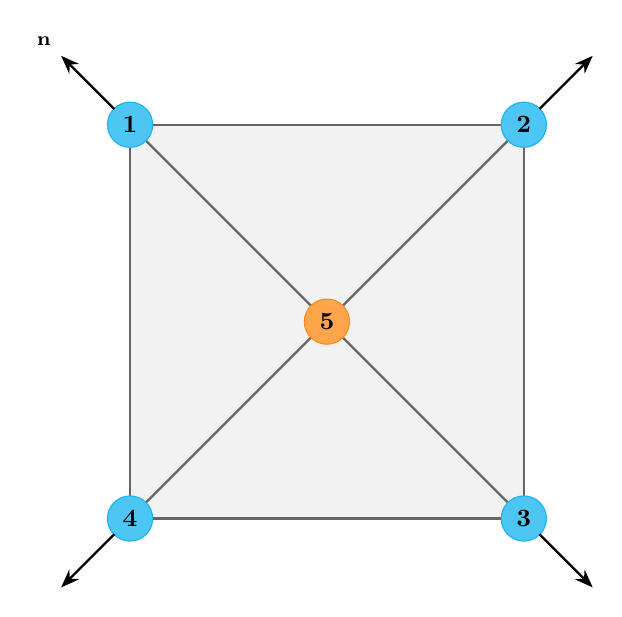
\begin{tikzpicture}[
    scale=2.5,
    >=Stealth,
    boundary node/.style={circle,fill=cyan!70,draw=cyan!90,inner sep=3pt,font=\small\bfseries},
    internal node/.style={circle,fill=orange!70,draw=orange!90,inner sep=3pt,font=\small\bfseries},
    mesh edge/.style={black!60,thick},
    normal vector/.style={->,thick,black}
]

% Domínio (quadrado)
\draw[mesh edge,fill=gray!10] (0,0) rectangle (2,2);

% Nós de fronteira
\coordinate (n1) at (0,2);
\coordinate (n2) at (2,2);
\coordinate (n3) at (2,0);
\coordinate (n4) at (0,0);

% Nó interno
\coordinate (n5) at (1,1);

% Arestas internas conectando ao nó central
\draw[mesh edge] (n1) -- (n5);
\draw[mesh edge] (n2) -- (n5);
\draw[mesh edge] (n3) -- (n5);
\draw[mesh edge] (n4) -- (n5);

% Triângulos
\draw[mesh edge] (n1) -- (n2);
\draw[mesh edge] (n2) -- (n3);
\draw[mesh edge] (n3) -- (n4);
\draw[mesh edge] (n4) -- (n1);

% Desenhar nós
\node[boundary node] at (n1) {1};
\node[boundary node] at (n2) {2};
\node[boundary node] at (n3) {3};
\node[boundary node] at (n4) {4};
\node[internal node] at (n5) {5};

% Vetores normais nas fronteiras (originando da borda dos círculos)
% Raio do círculo aproximado: 3pt * scale = 3pt * 2.5 = 7.5pt ≈ 0.06 unidades
\draw[normal vector] ($(n1) + (-0.08,0.08)$) -- ($(n1) + (-0.35,0.35)$) node[above left,font=\scriptsize] {$\mathbf{n}$};
\draw[normal vector] ($(n2) + (0.08,0.08)$) -- ($(n2) + (0.35,0.35)$);
\draw[normal vector] ($(n3) + (0.08,-0.08)$) -- ($(n3) + (0.35,-0.35)$);
\draw[normal vector] ($(n4) + (-0.08,-0.08)$) -- ($(n4) + (-0.35,-0.35)$);

\end{tikzpicture}
\end{document}
